
%%%%%%%%%%%%%%%%%%%%%%%%%%%%%%%%%%%%%%%%%%%%%%%%%%%%%%%%%%%%%%%%%%%%%%%%%%%%%
%%%%%%%%%%%%%%%%%%%%%%%%%%%%%%%%%%%%%%%%%%%%%%%%%%%%%%%%%%%%%%%%%%%%%%%%%%%%%
\chapter{HIDDEN MARKOV MODELS}

Hidden Markov Models are based on over hundred years old mathematical construct
called Markov Chains (MC). An MC can be in one of distinct $N$ states and the
transition between those states occur according to predefined transition
probabilities at discrete intervals. For the simplest, first-order Markov Chain,
these probabilities can be captured in a \PVerb!NxN!  matrix. The fact that
present state is enough to represent a system and is the only factor that
determines the future (through the transition table) is also called as the
system having the ``Markov property''. This also means that given present state,
the past and future are independent of eachother. Mathematically, a Markov Chain
is a sequence of random variables $X_1,X_2,X_3,...$, the state of the system at
time $t$ being $x_t$, then
\begin{eqnarray*}
P(X_{t+1} = x | X_t = x_t,...,X_1=x_1) = P(X_{t+1} = x | X_t = x_t)
\end{eqnarray*}
A Markov Chain could also be second order or third order and so on - for example
for second order Markov Chains, the transition table is \PVerb!2N x N! which
necessitates both present and {\em previous} step to obtain a transition probability
distribution for the next state.

Markov Chains have no hidden states. The emissions are the states themselves,
the transition probability matrix captures all the dynamics of the system. HMMs
improve on this model by adding a second layer of probability distribution that
represents observation values.

We assume a two level structure, with one level for hidden states, another for
observed states. Observed states model the ``emissions'', the output of the
model. In a typical setting where HMMs are used for prediction, modeler needs to
supply the number hidden states - an optimal value for this is usually
determined by using seperate training sets. 

Hidden and observed states have different distributions.

\begin{figure}[!hbp]
\center{
  \scalebox{0.8}{
  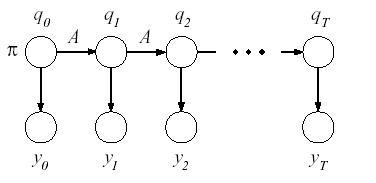
\includegraphics{./hmm/hmm-intro.jpg}
  }
}
\caption{Hidden and observed states of an HMM}
\vspace{0.6cm}
\end{figure}


Following the style and derivations by Bishop and Jordan \cite{jordan}, hidden
states sequence which correspond to an observation sequence are represented as
$q_1,...,q_T$. The output sequence is represented by random variables
$y_1,...,y_T$ where $T$ represents the number of available data points. It will
be assumed that $q_t$ and $y_t$ are i.i.d $\forall t$ , that is, as time
progresses, the underlying distribution will not change for $q_t$ and
$y_t$. There is a conditional dependence between $y_t$ and $q_t$, $q_t$ and
$q_{t-1}$. 

\begin{figure}[!hbp]
\center{
  \scalebox{0.8}{
  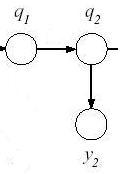
\includegraphics{./hmm/hmm-dep.jpg}
  }
}
\caption{Dependency between nodes of an HMM}
\vspace{0.6cm}
\end{figure}

We let random variable $q_t$ to have a multinomial distribution. There are $M$
finite states and for $q_t$ at state $i$, the``output'' of $q_t$ is a vector of
size M carrying a ``1'' at index i, ``0'' otherwise. Another representation that
can be used is $q_t^i = 1$ where $i \in \{1,..,M\}$ and $p(q_t)$ being a vector
of size $M$ where each cell carries the probability value for a possible value
of $q_t$.

There is conditional dependency between $y_t$ and $q_t$, and $q_t$ and
$q_{t-1}$. Since $q_t$ is multinomial, and there are $M$ states, joint
distribution between $q_t$ and $q_{t-1}$ should be represented by a table of
size $M$ x $M$. Let's call this $M$ x $M$ table the transition matrix
$A$. $a_{ij}$ gives transition probability $p(q_t^j=1 | q_t^i=1)$. Notice A is
independent of $t$.

Data output is captured in $y_t$. Output probability is $p(y_t|q_t)$. We make no
assumptions on this distribution for now. 

One of our goals with HMM will be training it with ``given'' emissions (output)
$y_1,..,y_T$ to come up with matrix $A$ which can also be represented as
$p(q_t^j=1 | q_t^i=1)$. Another goal of HMM use is being able to compute a
likelihood - given a matrix $A$ and observation sequence $y$ we should be able
to compute the likelihood of a ``hidden'' state sequence $q$, more succintly
$p(q|y)$.

It's easier to compute $p(q_t|y)$ instead of entire $q$. We can use $p(y|q_t)$
to get to $p(q_t|y)$.
\begin{eqnarray*}
p(q_t|y) &=& \frac{p(y|q_t) p(q_t)}{p(y)}
\end{eqnarray*}
Then, we need to calculate $p(y|q_t)$ and $p(y)$. Trick: Conditioning rule
states given $q_t$,
\begin{itemize}
   \item $q_{t-1}$ becomes independent of $q_{t+1}$
   \item $y_{t-1}$ becomes independent of $y_{t+1}$.
\end{itemize}


% proofs were conditional indep were here see proofs.tex

\begin{eqnarray*}
p(q_t|y) &=& \frac{p(y|q_t) p(q_t)}{p(y)}\\
&=& \frac{p(y_0...y_t|q_t)p(y_{t+1}...y_T|q_t) p(q_t)}{p(y)}\\
&=& \frac{p(y_0...y_t,q_t)p(y_{t+1}...y_T|q_t)}{p(y)}\\
p(q_t|y) &=& \frac{\alpha(q_t)\beta(q_t)}{p(y)}
\end{eqnarray*}
where
\begin{eqnarray*}
\alpha(q_t) & \triangleq & p(y_0...y_t,q_t) \\
\beta(q_t) & \triangleq & p(y_{t+1}...y_T|q_t)
\end{eqnarray*}
Obtain $p(y)$ by applying $\sum_{q_t}$ on both sides
\begin{eqnarray}
\sum_{q_t}p(q_t|y)  &=& \sum_{q_t} \frac{\alpha(q_t)\beta(q_t)}{p(y)} \nonumber\\
1  &=& \sum_{q_t} \frac{\alpha(q_t)\beta(q_t)}{p(y)} \nonumber\\
p(y) &=& \sum_{q_t} \alpha(q_t)\beta(q_t) \label{py}
\end{eqnarray}

\section{Forward-Backward Recursion}

We are finished with $p(y)$. We can move on to $\alpha(q_t)$ and
$\beta(q_t)$. We will compute these recursively. That is, from $\alpha(q_t)$ we
will compute $\alpha(q_{t+1})$.

\begin{eqnarray*}
\alpha(q_{t+1}) &=& p(y_0,...,y_{t+1},q_{t+1}) \\
 &=& p(y_0,...,y_{t+1}|q_{t+1})p(q_{t+1})\\
 &=& p(y_0,...,y_t|q_{t+1})p(y_{t+1}|q_{t+1})p(q_{t+1})\\
 &=& p(y_0,...,y_t,q_{t+1})p(y_{t+1}|q_{t+1})\\
 &=& \sum_{q_t}p(y_0,...,y_t,q_t,q_{t+1})p(y_{t+1}|q_{t+1})\\
 &=& \sum_{q_t}p(y_0,...,y_t,q_{t+1}|q_t)p(q_t)p(y_{t+1}|q_{t+1})\\
 &=& \sum_{q_t}p(y_0,...,y_t|q_t)p(q_{t+1}|q_t)p(q_t)p(y_{t+1}|q_{t+1})\\
 &=& \sum_{q_t}p(y_0,...,y_t,q_t)p(q_{t+1}|q_t)p(y_{t+1}|q_{t+1})\\
 &=& \sum_{q_t}\alpha(q_t)a_{q_t,q_{t+1}}p(y_{t+1}|q_{t+1})
\end{eqnarray*}
Similarly we can derive the equation for $\beta(q_t)$.
\begin{eqnarray*}
\beta(q_t) &=& p(y_{t+1},...,y_T|q_t) \\
&=& \sum_{q_{t+1}} p(y_{t+1},...,y_T,q_{t+1}|q_t) \\
&=& \sum_{q_{t+1}} \frac{p(y_{t+1},...,y_T,q_{t+1},q_t)}{p(q_t)}\\
&=& \sum_{q_{t+1}} \frac{p(y_{t+1},...,y_T,q_t|q_{t+1})p(q_{t+1})}{p(q_t)}\\
&=& \sum_{q_{t+1}} p(y_{t+1},...,y_T,q_t|q_{t+1})p(q_{t+1}|q_t)\\
&=& \sum_{q_{t+1}} p(y_{t+2},...,y_T,q_t|q_{t+1})p(q_{t+1}|q_t)p(y_{t+1}|q_{t+1})\\
&=& \sum_{q_{t+1}} \beta(q_{t+1}) a_{q_t,q_{t+1}} p(y_{t+1}|q_{t+1})
\end{eqnarray*}

We see that
\begin{itemize}
   \item $\alpha$ recursion is a forward recursion (we plug in $q_t$ to get
     $q_{t+1}$)
   \item $\beta$ recursion is a backward recursion (we plug in $q_{t+1}$ to get
     $q_{t}$)
\end{itemize}
The start-up equation can be calculated as follows:
\begin{eqnarray*}
\alpha({q_0}) &=& p(y_0,q_0)\\
&=& p(y_0|q_0)p(q_0)\\
&=& p(y_0|q_0)\pi_0
\end{eqnarray*}
There is a little complication for the start-up formula for $\beta$
recursion. In this case it would not be possible to start with $\beta(q_{T+1})$
because that state does not exist in our system. In this case, we can simply
start with vector of ones. For the proof the reader can refer to \cite{jordan}. 

% proof 2 buradaydi

% EM param estimation buradaydi
\section{Training}

We need to find optimal $\theta$ that maximizes $log (p(y,q|\theta))$ where
$\theta = (\pi,A,\eta)$. We know $\pi$ and $A$. $\eta$ represents parameters
necessary for $p(y_t|q_t)$, the output distribution.

Let's write the full $p(y,q)$ distribution;
\begin{eqnarray*}
p(q,y) &=& \pi_{q_0} \prod_{t=0}^{T-1} a_{q_t,q_{t+1}} \prod_{t=0}' p(y_t|q_t,\eta)
\end{eqnarray*}
We take log, use Lagrange multipliers, take derivative set to zero and solve:
{\small
\begin{eqnarray*}
\hat{a}_{ij}  &=& \frac{\sum_{t=0}^{T-1} q_t^i q_{t+1}^j}{\sum_{j=1}^M \sum_{t=0}^{T-1} q_t^i q_{t+1}^j} 
\end{eqnarray*}}
Similarly for $\eta_{ij}$ and $\pi_i$,
\begin{eqnarray*}
\hat{\eta}_{ij} &=& \frac{\sum_{t=0}^{T-1} q_t^i y_t^j}{\sum_{k=1}^N
\sum_{t=0}^{T-1} q_t^i y_t^k} \\
\hat{\pi}_i &=& q_0^i
\end{eqnarray*}

$\hat{\eta}_{ij}$ assumes a multinomial output distribution $y_t$. For stock
prediction purposes, we will be using a Gaussian distribution to represent
each stock price at time $t$. Therefore, we can simply use $y_t$ itself as the
output instead of the $y_t^j$, hence $\hat{\eta}$ changes to being the mean of
the estimated Gaussian.
\begin{eqnarray*}
\hat{C}_{i}^{(p+1)} &=& \frac{\sum_{t=0}^T\gamma_{t}^i y_t}{\sum_{t=0}^T\gamma_{t}^i}
\end{eqnarray*}
where $\gamma_{t}$ is the posterior probability $p(q_t|y)$ at time $t$.

In each iteration

\begin{itemize}
   \item We calculate $\hat{a}$, $\hat{C}$, $\hat{R}$, $\hat{\pi}$ using given
     $q$ and $y$.
   \item We calculate $p(q_t|y)$ for each $q_t$ using $A$, $\eta$ and $\pi$ using
   forward backward recursion.
\end{itemize}

\section{Algorithm}

The algorithm for HMM forward-backward inference and training through EM
(Baum-Welch) as presented by Roweis and Ghahramani \cite{ghahramani} can be
found below. The operator $\odot$ is defined to be element-wise product of two
equal size vectors or matrices. The algorithm assumes the emission distribution
is a multidimensional Gaussian.

\begin{figure}[!hbp]
\center{
\begin{tabbing}
 {\tt HMM}\={\tt Inference}\=(Y,A,$\pi$,C,R) \\
 {\tt for} t=1  to  T  \% forward pass \\
 \> {\tt for} i=1  to k \\
 \> \>$b_{t,i}=\texttt{exp}\{-\frac{1}{2}(y_t - C_i)'R^{-1}(y_t - C_i)\}|R|^{-1/2}(2\pi)^{-p/2}$\\
 \> {\tt end}\\
 \> if (t=1) $\alpha_t = \pi \odot b_1$ else $\alpha_t = [A'\alpha_{t-1}]\odot b_t$ end \\
 \> $\rho_t = \sum_i \alpha_{t,i}$\\
 \> $\alpha_t = \alpha_t / \rho_t$ \% normalization\\
 {\tt end}\\
 $\beta_T = 1/\rho_t$ \\
 {\tt for }t=T-1 to 1 \% backward pass \\
 \> $\beta_t = A[\beta_{t+1} \odot b_{t+1}]/ \rho_t$\\
 {\tt end}\\
 $\gamma_t = \alpha_t \odot \beta_t / (\alpha_t'\beta_t)$\\
 $\xi_t = \alpha_t[\beta_{t+1} \odot b_{t+1}]'$\\
 $\xi_t = \xi_t / (\sum_{ij}\xi_{ij})$\\
 {\tt return} $\gamma_t, \xi_t, \rho_t$ for all t
\end{tabbing}
}
\caption{HMM Inference Algorithm}
\vspace{0.6cm}
\end{figure}

\begin{figure}[!hbp]
\center{
\begin{tabbing}
{\tt HMM}\={\tt Lea}\={\tt rn}(Y,k,$\epsilon$) \\
\> {\tt initialize}  A, $\pi$, C, R \\
\> {\tt while change in log likelihood} $>$ $\epsilon$ \\
\> \> {\tt HMMInference}$(Y,A,\pi,C,R);$ \%E step\\
\> \> \% M Step\\
\> \> $\pi = \gamma_1$\\
\> \> $A = \sum_t \xi_t$\\
\> \> $A_{ij} = A_{ij} / \sum_l A_{il}$ {\tt for all }$ i,j$\\
\> \> $C_j = \sum_t \gamma_{t,j} y_t / \sum_t \gamma_{t,j}$ {\tt for all } $j$\\
\> \> $R = \sum_{t,j} \gamma_{t,j} (y_t - C_j)(y_t - C_j)' / T$\\
\> {\tt return } $A, \pi, C, R$
\end{tabbing}
}
\caption{HMM Learning Algorithm}
\vspace{0.6cm}
\end{figure}

%%%%%%%%%%%%%%%%%%%%%%%%%%%%%%%%%%%%%%%%%%%%%%%%%%%%%%%%%%%%%%%%%%%%%%%%%%%%%
\section{Prediction with HMM}

For HMMs, if we start generating using $\pi$, this would give us a replay of the
training data starting with day $1$, not future data starting at $T+1$. Then, we
should not start generating starting with $\pi$, instead, we need to determine
{\em the last hidden state of our HMM} on day $T$, and use transition table $A$
to get to hidden state at day $T+1$, {\em then} we can start generating predictions.

In order to find the hidden state at day $T$, we can simply run the Viterbi
algorithm that gives us the most likely hidden path for the given data and given
HMM. Then, we simply pick the last element from this list, roll the dice and
apply transition once, and this gives us our first prediction for day $T+1$. The
rest will be the same as generating data from a regular HMM - we keep following
the transition table. The pseucode for the function
\PVerb!observationGeneration!  looks as follows:

\begin{figure}[!hbp]
\center{
\begin{tabbing}
{\tt obser}\={\tt vation}\={\tt Genera}\={\tt tion}$(A,\pi,C,R,N)$\\
\> $states$ = {\tt viterbi}($A,\pi,C,R$);\\
\> $lastState = states[T]$;\\
\> {\tt } for $i = 1$ {\tt to } $N$\\
\> \> $currentState = {\tt nextState}(lastState,A,\pi,C,R);$\\
\> \> $mean = C[currentState]$;\\
\> \> $variance = R[currentState];$\\
\> \> $o[i] = $ {\tt gaussianRandomGeneration}$(mean,variance);$\\
\> \> $lastState = currentState;$\\
\> {\tt end}\\
\> {\tt return} $o$;
\end{tabbing}
}
\caption{Algorithm for Generating Observations}
\vspace{0.6cm}
\end{figure}

\newpage

\begin{figure}[ht]
\center{
\begin{tabbing}
{\tt next}\={\tt Sta}\={\tt te}$(stat$\=$e,A,\pi,C,R);$\\ 
\> $randVal = ${\tt generateUniform(0,1);}\\
\> $total = 0;$\\
\> $done = false;$\\
\> $total = A[currentState][0];$\\
\> {\tt for } $j = 1$ {\tt to } $numStates$\\
\> \> {\tt if} $done = true$ {\tt break};\\
\> \> {\tt if} $(randVal > total$ {\tt and } \\
\> \> \> $randVal \leqslant (total + A[currentState][j]))$\\
\> \> \> $currentState = j;$\\
\> \> \> $done = true;$\\
\> \> {\tt end}\\
\> \> $total = total+ A[currentState][j]$;\\
\> {\tt end}\\
\> {\tt return} $currentState$;
\end{tabbing}
}
\caption{State Transition Algorithm}
\vspace{0.6cm}
\end{figure}
